%!TEX root = ../../thesis.tex

Utilising the measurement methods used previously, a liquid that better replicates a biological impedance is sought.
This work is of benefit to engineers of medical implant devices.
Having the ability to formulate a solution that mimics the electrical conditions inside a living mammal reduces the resources required to test electronic implants.

It was previous mentioned that the developers of spinal cord stimulator implants used solutions of PBS having a one-tenth concentration as a test fluid for their implants.
This solution was the best substitute for an actual live spine that these engineers had.
Solutions of the \SI{0.1}{X} PBS were held in drums within the electronics laboratories for use whenever a quick tests needed to be carried out.
Electrodes were submerged into these buckets in order to recreate the electrical conditions inside a human spine.

This was not the only way to simulate the impedance conditions inside a person.
As presented in~\cref{sect:sheep_measurements}, the use of anaesthetised sheep were also used.
A sheep's spine is smaller than a human's but is a good approximation in term of geometry.
However, the resources involved with conducting a live sheep trial are high; requiring use of a hospital operating theatre, surgeon veterinarian, and equipment.

Engineers had no way of knowing how well those baths of saline represented a sheep's spine.
It was shown in \cref{sect:sheep_measurements} that the match between the two was weak.
With that knowledge, and the measurement techniques developed thus far, research into creating a solution that better matches sheep spine is carried out.
Such a match would reduce the number of surgical operations the test engineers might need to conduct, saving resources and reducing time.


\section{Measurement}


  The function generator, Agilent 33220A, and oscilloscope, Tektronix TPS 2024, are connected to the electrode array, St. Jude Medical - Octrode, as is shown in \cref{fig:creatingCSF_setup}.
  A \SI{10}{\kilo\ohm} resistor was used to measure the current driven between electrodes eight and three.
  It had a measured resistance of \SI{9.990}{\kilo\ohm}, as measured with a Fluke Digital Multimeter.

  \begin{figure}
      \centering
      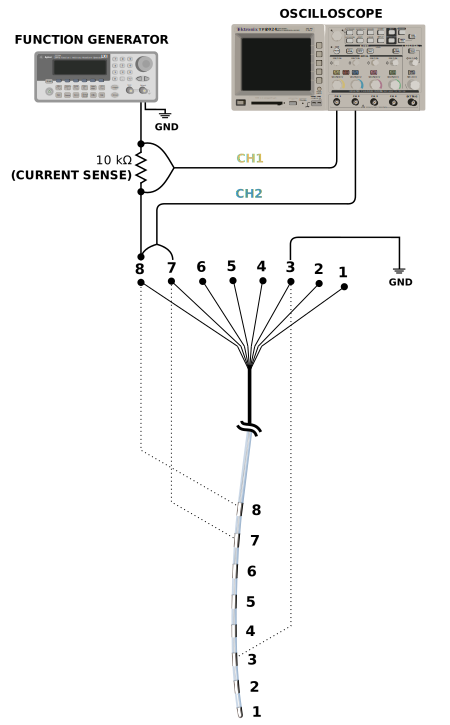
\includegraphics[scale=0.95]{content/pt2/graphics/CreatingCSF_setup}
      \caption{\label{fig:creatingCSF_setup}Diagram showing the measurement configuration used to measure the CPE response and resistivity of mixed solutions}
  \end{figure}

  Each measurement run begin at the upper end of the frequency spectrum and proceeded towards the low frequency endpoint.
  Starting with the higher frequencies offers a chance to confirm correct measurement set-up early in the measurement.
  A sample at the lowest frequency can take over a minute to acquire, where the higher frequencies drop to under a second.
  The same frequencies were chosen that were used to measure the situation in live sheep.
  This allows easy comparison between the sheep data and the impedance of mixed solutions.

  Measurements were completely automated via a Linux based computer running Python scripts.
  These scripts controlled the output settings of the waveform generator and acquired the resulting waveforms from the oscilloscope.
  The scripts had the ability to set the horizontal and vertical scales on the oscilloscope channels in order to ensure appropriate scales were used.

  \begin{figure}
      \centering
      
\includegraphics[width=\textwidth]{content/pt2/graphics/measurementFlowchart}
      \caption{\label{fig:creatingCSF_pythonFlowchart}Diagram showing the execution of the measurement script}
  \end{figure}

  The measurement procedure followed by the script is shown as a simplified flowchart in \cref{fig:creatingCSF_pythonFlowchart}.
  The programme steps through each of the required frequencies, making sure the target voltage is developed across electrodes seven and eight, calculating the interface impedance.

  The target voltage across the interface is \SI{20}{\milli\volt}.
  This voltage was previously determined as a safe stimulus voltage in that it does not trigger Faradaic reactions at the electrode's surface.
  Because the impedance of the interface changes with frequency, it is necessary to alter the output amplitude to keep the voltage across electrode seven and eight consistent.

  This measurement configuration differs from the three channel method used in earlier measurements.
  Those used channel three of the oscilloscope to watch the voltage developed between electrodes three and eight.


\section{Ingredients}


  To determine how certain additives affect the impedance of the interface, a range of ingredients were mixed and tested.
  Various mixtures were created in a trial-and-error fashion until trends emerged which eliminated many of the ingredients.
  The following ingredients were tried for mixture creation:
  \begin{itemize}
      \item Glycerol
      \item Methylated Spirits
      \item Sodium Carbonate
      \item Sodium Bicarbonate
      \item Table-salt (non-iodised)
      \item Gelatine
      \item Citric Acid
      \item Corn-flour
  \end{itemize}


% \section{Results}


%  \subsection{Water, Corn-flour and Salt}
%
%    \begin{figure}
%        \centering
%        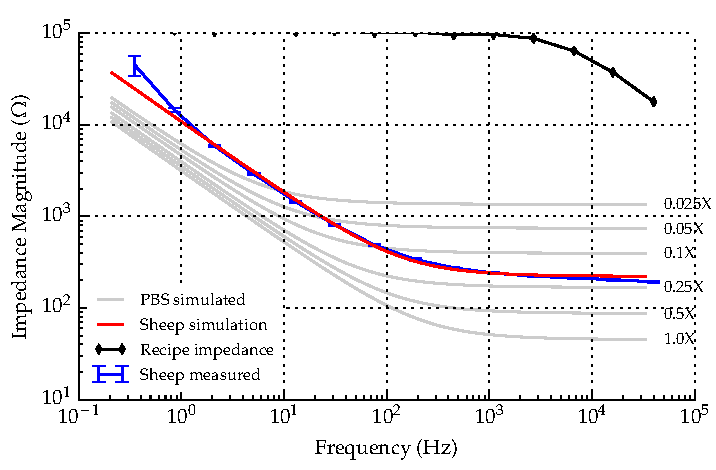
\includegraphics[width=\textwidth]{content/pt2/graphics/run12_600ml-distilledWater_ZVsF_graph_mag}
%        \caption{\label{fig:recipe_water_mag}Plot of impedance magnitude versus frequency (log-log) for distilled water.}
%    \end{figure}
%
%    \begin{figure}
%        \centering
%        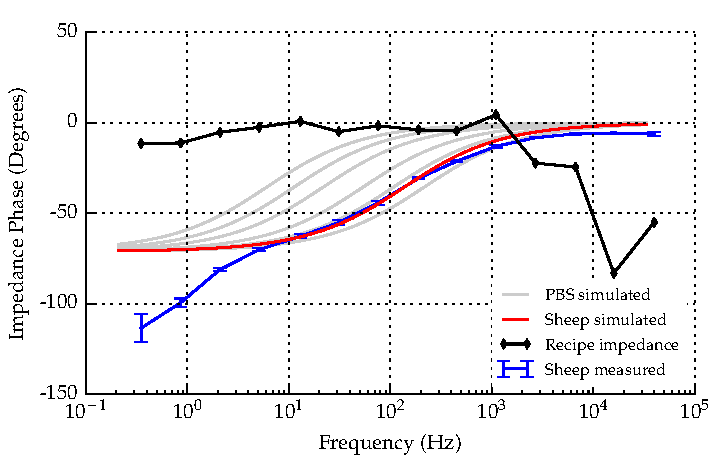
\includegraphics[width=\textwidth]{content/pt2/graphics/run12_600ml-distilledWater_ZVsF_graph_phase}
%        \caption{\label{fig:recipe_water_phase}Plot of impedance phase versus frequency (log-log) for distilled water.}
%    \end{figure}
%
%    \begin{figure}
%        \centering
%        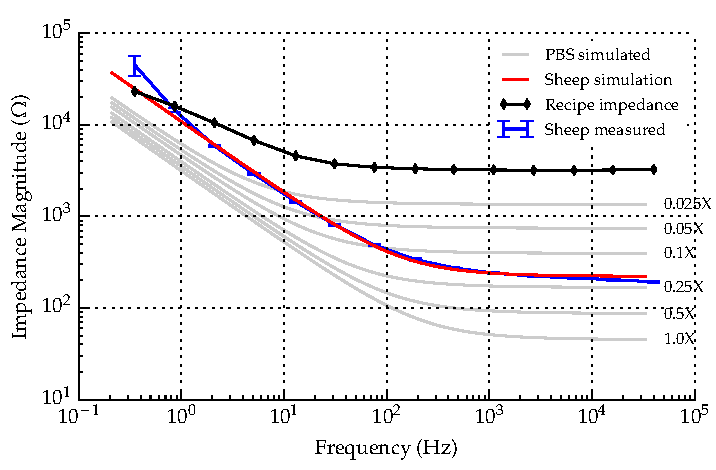
\includegraphics[width=\textwidth]{content/pt2/graphics/run14_170ml-distilledWater_250g-cornflour_ZVsF_graph_mag}
%        \caption{\label{fig:recipe_cornflour_mag}Plot of impedance magnitude versus frequency (log-log) for \SI{250}{\gram} cornflour mixed with \SI{175}{\milli\litre} distilled water.}
%    \end{figure}
%
%    \begin{figure}
%        \centering
%        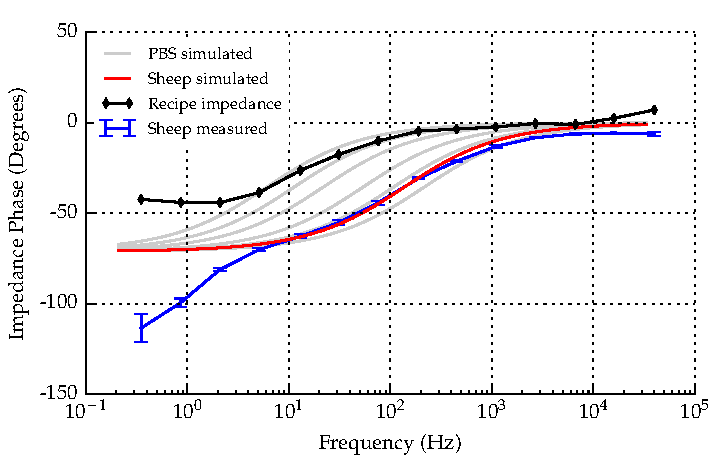
\includegraphics[width=\textwidth]{content/pt2/graphics/run14_170ml-distilledWater_250g-cornflour_ZVsF_graph_phase}
%        \caption{\label{fig:recipe_cornflour_phase}Plot of impedance phase versus frequency (log-log) for \SI{250}{\gram} cornflour mixed with \SI{175}{\milli\litre} distilled water.}
%    \end{figure}
%
%    \begin{figure}
%        \centering
%        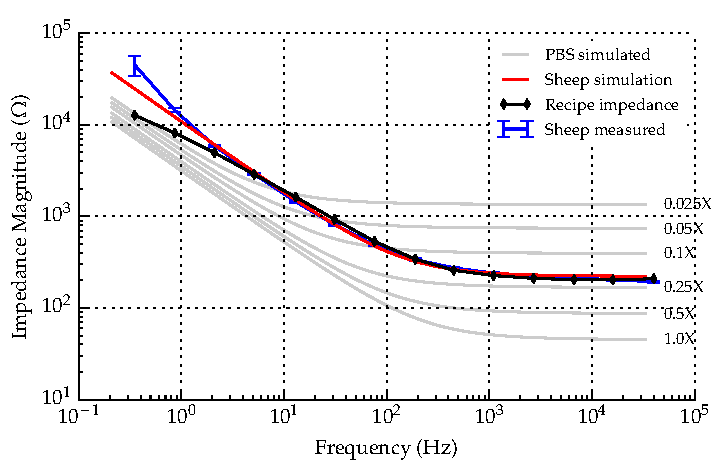
\includegraphics[width=\textwidth]{content/pt2/graphics/run14_175ml-distilledWater_250g-cornflour_1g9-salt_ZVsF_graph_mag}
%        \caption{\label{fig:recipe_cornflour_salt_mag}Plot of impedance magnitude versus frequency (log-log) for \SI{250}{\gram} cornflour mixed with \SI{175}{\milli\litre} distilled water and \SI{1.9}{\gram} table-salt.}
%    \end{figure}
%
%    \begin{figure}
%        \centering
%        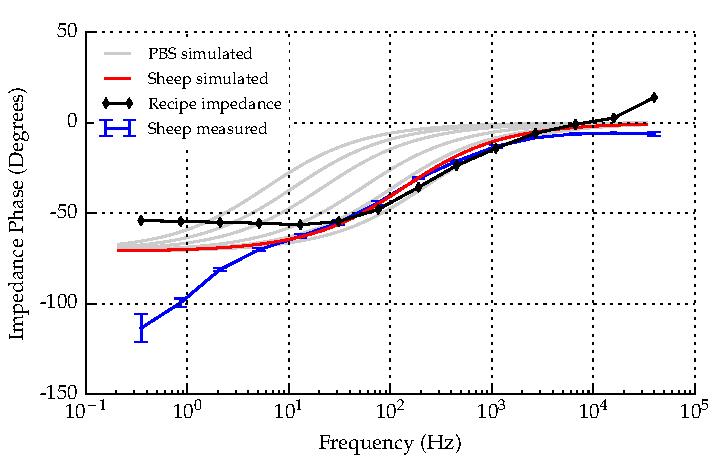
\includegraphics[width=\textwidth]{content/pt2/graphics/run14_175ml-distilledWater_250g-cornflour_1g9-salt_ZVsF_graph_phase}
%        \caption{\label{fig:recipe_cornflour_salt_phase}Plot of impedance phase versus frequency (log-log) for \SI{250}{\gram} cornflour mixed with \SI{175}{\milli\litre} distilled water and \SI{1.9}{\gram} table-salt.}
%    \end{figure}
%
%    \begin{figure}
%        \centering
%        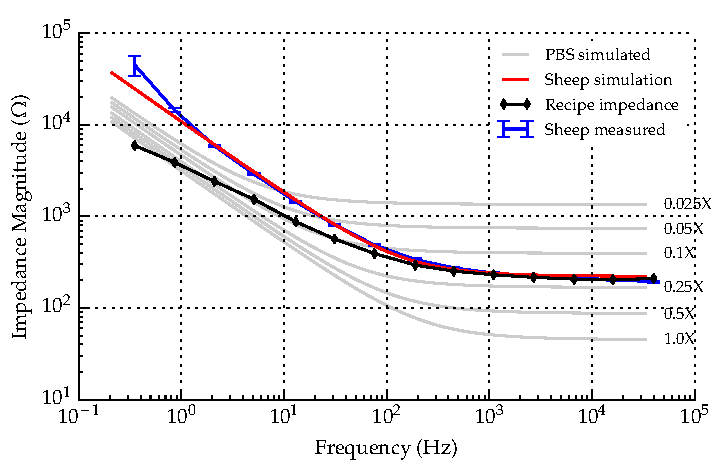
\includegraphics[width=\textwidth]{content/pt2/graphics/run14_180ml-distilledWater_250g-cornflour_1g9-salt_ZVsF_graph_mag}
%        \caption{\label{fig:recipe_cornflour_salt_extraWater_mag}Plot of impedance magnitude versus frequency (log-log) for \SI{250}{\gram} cornflour mixed with \SI{180}{\milli\litre} distilled water and \SI{1.9}{\gram} table-salt.}
%    \end{figure}
%
%    \begin{figure}
%        \centering
%        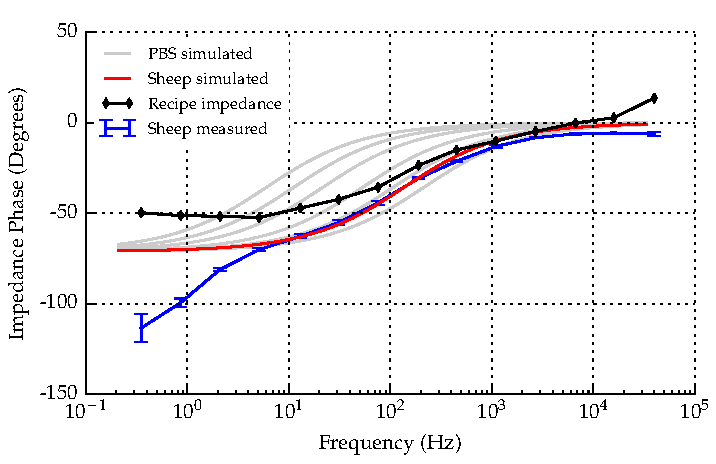
\includegraphics[width=\textwidth]{content/pt2/graphics/run14_180ml-distilledWater_250g-cornflour_1g9-salt_ZVsF_graph_phase}
%        \caption{\label{fig:recipe_cornflour_salt_extraWater_phase}Plot of impedance phase versus frequency (log-log) for \SI{250}{\gram} cornflour mixed with \SI{180}{\milli\litre} distilled water and \SI{1.9}{\gram} table-salt.}
%    \end{figure}
%
%    \Cref{fig:recipe_water_mag,fig:recipe_water_phase,fig:recipe_cornflour_phase,fig:recipe_cornflour_mag,fig:recipe_cornflour_phase,fig:recipe_cornflour_salt_mag,fig:recipe_cornflour_salt_phase,fig:recipe_cornflour_salt_extraWater_mag,fig:recipe_cornflour_salt_extraWater_phase} show a progression of measurements beginning with distilled water, then adding cornflour, then adding salt, and finally adding a very small amount of extra water.

\section{Results \& Discussion}

  \begin{figure}
      \centering
      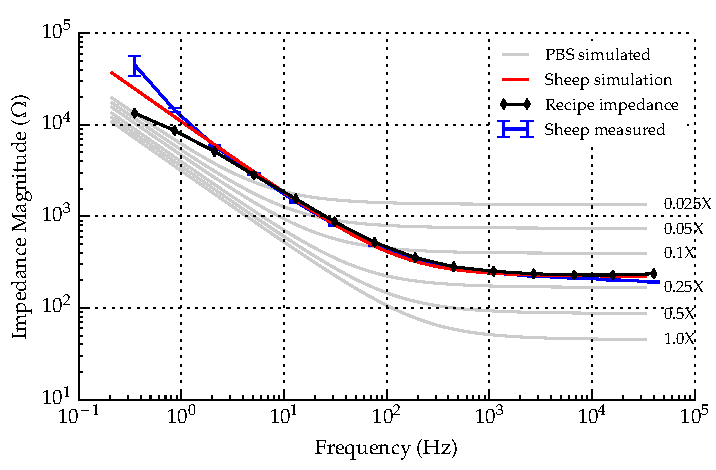
\includegraphics[width=\textwidth]{content/pt2/graphics/run12_190ml-distilledWater_190g-cornflour_0g858-salt_ZVsF_graph_mag}
      \caption{\label{fig:recipe_cornflour_salt_extraWater_mag_improved}Graph of measured impedance magnitude versus frequency (log-log) for \SI{190}{\gram} cornflour mixed with \SI{190}{\milli\litre} distilled water and \SI{0.858}{\gram} table-salt.}
  \end{figure}

  \begin{figure}
      \centering
      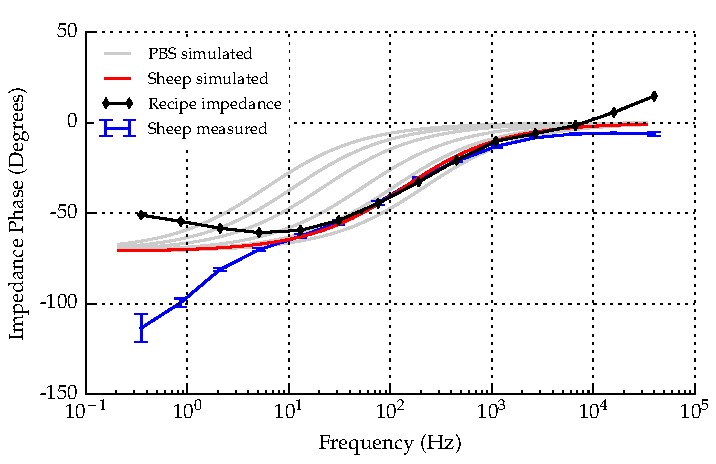
\includegraphics[width=\textwidth]{content/pt2/graphics/run12_190ml-distilledWater_190g-cornflour_0g858-salt_ZVsF_graph_phase}
      \caption{\label{fig:recipe_cornflour_salt_extraWater_phase_improved}Graph of impedance phase versus frequency (log-log) for \SI{190}{\gram} cornflour mixed with \SI{190}{\milli\litre} distilled water and \SI{0.858}{\gram} table-salt.}
  \end{figure}

  \Cref{fig:recipe_cornflour_salt_extraWater_mag_improved,fig:recipe_cornflour_salt_extraWater_phase_improved} show the results of mixing the same set of ingredients as the previous measurement set, but with the closest fit to sheep spine obtained.


%\section{Discussion}


  These results show that it is possible to alter the CPE response and the bulk conductivity of the solution independently of one another.
  \Cref{fig:recipe_cornflour_salt_extraWater_mag_improved,fig:recipe_cornflour_salt_extraWater_phase_improved} show a greatly improved match relative to that of any single concentration of PBS.
  Unbuffered saline solutions all dipped in impedance magnitude at low frequencies, something not observed when using buffered saline such as PBS.
  It is expected that using buffered saline solutions would bring the low-frequency response back in line with the PBS trace.
  It may also be possible to select an appropriate buffering agent that better matches the response of the sheep's biological fluid.
  These results are promising and no doubt will be of use not only to implant designers but to anyone trying to mimic the electrical impedance of biological fluids.
